\chapter{Kiểm thử phần mềm}

\section{Kiểm thử Frontend}

Nhóm đã kiểm thử frontend ở mức unit, context, component và service contract
bằng Jest, Testing Library và môi trường \texttt{jsdom}. Mục tiêu của phần kiểm
thử này là bắt các lỗi dễ tái xuất hiện trong giao diện: ánh xạ lỗi nghiệp vụ từ
backend sang thông báo người dùng, trạng thái đăng nhập, đa ngôn ngữ Việt--Anh,
light/dark/system theme, upload panel, nội dung notification, Google Maps ở
trang liên hệ, service layer gọi đúng endpoint, admin audit/policy contract và
các helper xử lý trạng thái đặt trước.

Khác với kiểm thử thủ công chỉ quan sát giao diện, các test này kiểm tra trực
tiếp logic dùng chung trong \texttt{utils} và \texttt{contexts}. Đây là những
vị trí có phạm vi ảnh hưởng rộng: nếu \texttt{LanguageContext} sai, nhiều trang
bị sai ngôn ngữ; nếu \texttt{ThemeContext} sai, toàn bộ SPA bị lệch theme; nếu
\texttt{getFriendlyErrorMessage} sai, cùng một lỗi backend có thể bị hiển thị
thành thông báo không đúng nghiệp vụ. Ngoài ra, các test service contract giúp
nhóm kiểm soát URL, query string và payload gửi về backend/AI service trước khi
chạy tích hợp thật.

\subsection{Môi trường và cấu hình kiểm thử}

Frontend dùng \texttt{jest.config.cjs} để chạy các file
\texttt{*.test.ts} và \texttt{*.test.tsx}. Môi trường \texttt{jsdom} được chọn
vì các context cần thao tác với \texttt{localStorage}, \texttt{document.html},
\texttt{matchMedia} và DOM giống trình duyệt. File \texttt{src/test/setup.ts}
nạp \texttt{@testing-library/jest-dom} để assertion có thể viết gần với hành vi
giao diện hơn, ví dụ \texttt{toHaveTextContent} và \texttt{toHaveClass}.

\begin{table}[H]
\centering
\small
\begin{tabularx}{\textwidth}{|p{3.5cm}|X|}
\hline
\textbf{Thành phần} & \textbf{Cấu hình sử dụng} \\
\hline
Test runner & Jest, chạy bằng script \texttt{npm test -- --runInBand}. \\
\hline
Biên dịch test & \texttt{ts-jest} với JSX mode \texttt{react-jsx}. \\
\hline
Môi trường DOM & \texttt{jest-environment-jsdom}, hỗ trợ kiểm tra DOM, \texttt{localStorage} và \texttt{document}. \\
\hline
Assertion UI & \texttt{@testing-library/jest-dom}. \\
\hline
Mock style & \texttt{identity-obj-proxy} cho file CSS/SCSS. \\
\hline
Alias import & \texttt{@/(.*)} trỏ về thư mục gốc frontend. \\
\hline
\end{tabularx}
\caption{Cấu hình kiểm thử Frontend}
\label{tab:fe_test_env}
\end{table}


\subsection{Phạm vi test đã hiện thực}

Nhóm ưu tiên các phần logic có khả năng ảnh hưởng nhiều màn hình thay vì chỉ
kiểm từng nút bấm riêng lẻ. Bộ test cuối cùng bao phủ 11 suite, gồm logic dùng
chung, context toàn cục, component nhỏ, trang liên hệ và service layer.

\begin{table}[H]
\centering
\scriptsize
\begin{tabularx}{\textwidth}{|p{5.1cm}|X|p{1.5cm}|}
\hline
\textbf{File test} & \textbf{Nội dung kiểm thử} & \textbf{Số test} \\
\hline
\begin{tabular}[c]{@{}l@{}}\texttt{src/utils/}\\\texttt{errorMessages.test.ts}\end{tabular} &
Ánh xạ mã lỗi backend sang thông báo phù hợp cho duplicate email, duplicate review và text lỗi chung. & 4 \\
\hline
\begin{tabular}[c]{@{}l@{}}\texttt{src/utils/}\\\texttt{notification}\\\texttt{Localization.test.ts}\end{tabular} &
Localize notification theo ngôn ngữ, giữ dữ liệu động như tên sách, số tiền và vị trí hàng chờ. & 3 \\
\hline
\begin{tabular}[c]{@{}l@{}}\texttt{src/utils/}\\\texttt{reservationUtils.test.ts}\end{tabular} &
Nhãn/màu trạng thái đặt trước, format ngày, quyền hủy reservation và deadline nhận sách. & 18 \\
\hline
\begin{tabular}[c]{@{}l@{}}\texttt{src/contexts/}\\\texttt{LanguageContext}\\\texttt{.test.tsx}\end{tabular} &
Ngôn ngữ mặc định, fallback text, chuyển sang English, lưu \texttt{localStorage} và cập nhật \texttt{document.lang}. & 2 \\
\hline
\begin{tabular}[c]{@{}l@{}}\texttt{src/contexts/}\\\texttt{ThemeContext}\\\texttt{.test.tsx}\end{tabular} &
Theme mặc định \texttt{system}, dark/light mode, \texttt{prefers-color-scheme}, class \texttt{dark} trên thẻ \texttt{html}. & 3 \\
\hline
\begin{tabular}[c]{@{}l@{}}\texttt{src/contexts/}\\\texttt{AuthContext.test.tsx}\end{tabular} &
Load role đã lưu, login bằng mật khẩu/social, parse role từ JWT và logout xóa token. & 5 \\
\hline
\begin{tabular}[c]{@{}l@{}}\texttt{src/contexts/}\\\texttt{UploadContext}\\\texttt{.test.tsx}\end{tabular} &
Thêm/cập nhật/xóa upload, progress/status và cảnh báo \texttt{beforeunload} khi upload đang chạy. & 5 \\
\hline
\begin{tabular}[c]{@{}l@{}}\texttt{src/components/}\\\texttt{UiComponents.test.tsx}\end{tabular} &
Star rating, password visibility toggle và disabled button. & 3 \\
\hline
\begin{tabular}[c]{@{}l@{}}\texttt{src/components/}\\\texttt{Switchers.test.tsx}\end{tabular} &
Language switcher và theme mode toggle thao tác đúng context toàn cục. & 2 \\
\hline
\begin{tabular}[c]{@{}l@{}}\texttt{src/pages/}\\\texttt{ContactPage.test.tsx}\end{tabular} &
Thông tin liên hệ, iframe Google Maps lazy loading và submit form liên hệ. & 2 \\
\hline
\begin{tabular}[c]{@{}l@{}}\texttt{src/api/}\\\texttt{frontendServices.test.ts}\end{tabular} &
Hợp đồng endpoint/payload cho search, semantic search, PayOS, wishlist, S3 upload, rating, admin audit, circulation policy, system review và ghi chú giao dịch. & 10 \\
\hline
\textbf{Tổng cộng} & \textbf{11 test suites} & \textbf{58} \\
\hline
\end{tabularx}
\caption{Các file test Frontend đã hiện thực}
\label{tab:fe_test_files}
\end{table}


\begin{figure}[H]
    \centering
    \IfFileExists{figures/ch07/test-results/fe-jest-result.png}{
        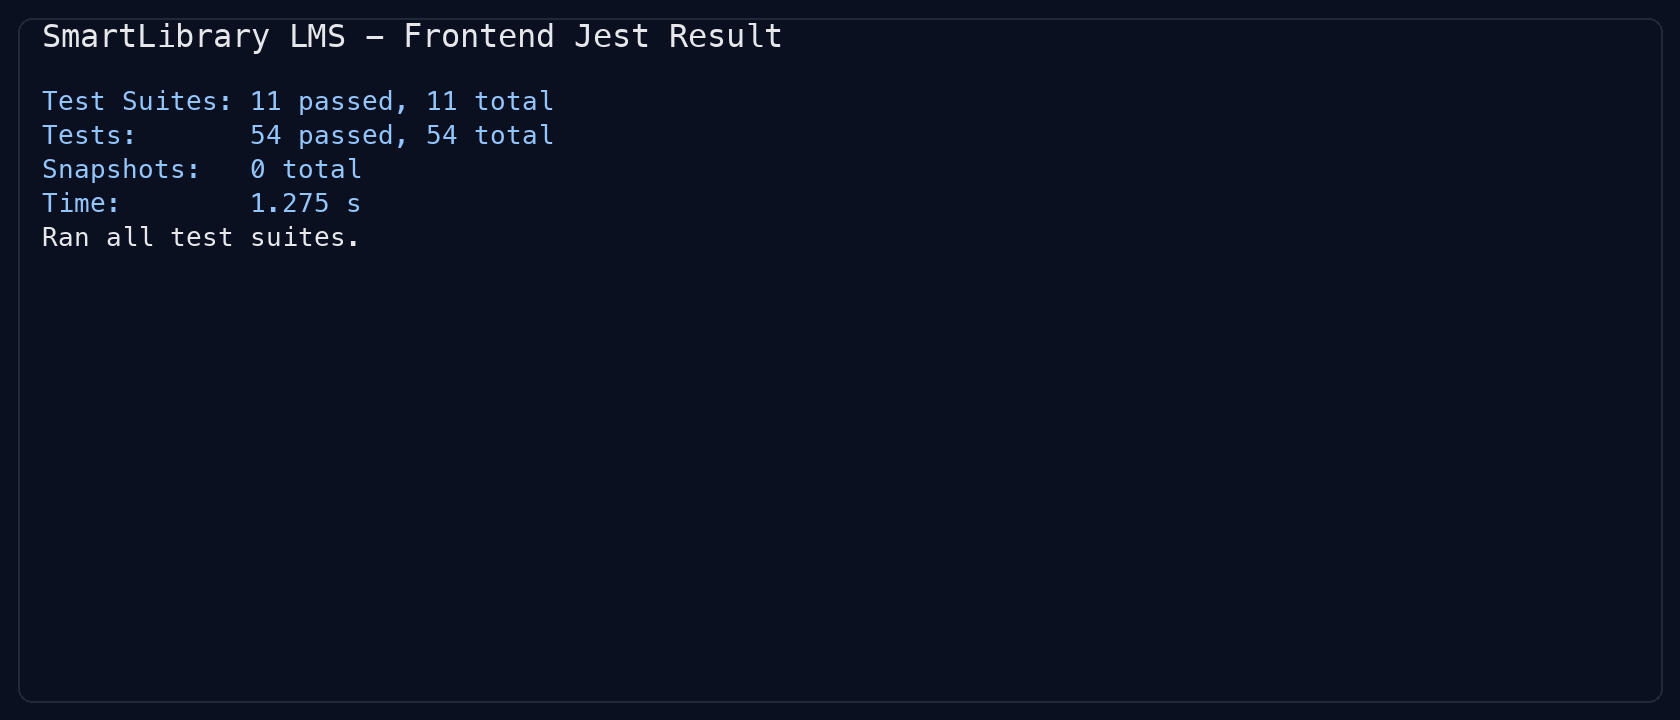
\includegraphics[width=0.9\textwidth]{figures/ch07/test-results/fe-jest-result.png}
    }{
        \fbox{\parbox[c][5cm][c]{0.9\textwidth}{\centering Placeholder: chạy \texttt{npm run test:report} trong \texttt{LMS\_fe} để tạo ảnh tại \texttt{figures/ch07/test-results/fe-jest-result.png}}}
    }
    \caption{Kết quả chạy unit/context test Frontend}
    \label{fig:fe_unit_test_result}
\end{figure}



\subsection{Kết quả thực thi}

Nhóm đã chạy lại bộ test frontend và đồng thời sinh ảnh kết quả bằng script
\texttt{test:report}

\begin{table}[H]
\centering
\small
\begin{tabularx}{\textwidth}{|p{4cm}|X|}
\hline
\textbf{Chỉ số} & \textbf{Kết quả} \\
\hline
Test suites & \textbf{11 passed / 11 total}. \\
\hline
Test cases & \textbf{58 passed / 58 total}. \\
\hline
Snapshot & \textbf{0 total}. \\
\hline
Thời gian chạy & Khoảng \textbf{1.424s} trên môi trường local. \\
\hline
Kết luận & Bộ test frontend pass toàn bộ ở tầng unit/context. \\
\hline
\end{tabularx}
\caption{Kết quả kiểm thử Frontend}
\label{tab:fe_test_result}
\end{table}

\subsection{Kiểm thử tích hợp Gemini thật}

Bên cạnh bộ regression offline, nhóm hiện thực kịch bản live để gọi Gemini thật
trên một PDF mẫu. Script \texttt{scripts/run\_live\_gemini\_report.py} đọc file
PDF bằng cùng hàm \texttt{extract\_pdf\_text}, chia chunk, gọi
\texttt{GeminiClient.reduce\_publication}, đo thời gian xử lý và ghi kết quả
JSON ra thư mục \texttt{figures/test-results}. Artifact JSON được thiết kế để
lưu các trường cần nghiệm thu: \texttt{master\_summary}, \texttt{tags},
\texttt{tags\_en}, \texttt{audience}, số chunk, số ký tự extract và thời gian
xử lý.


\begin{figure}[H]
    \centering
    \IfFileExists{figures/ch07/test-results/ai-gemini-live-result.png}{
        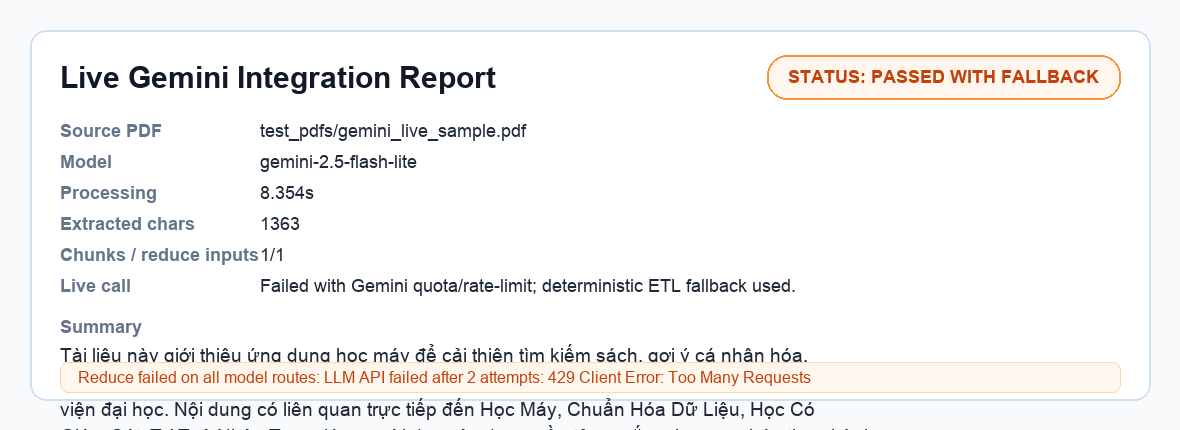
\includegraphics[width=0.9\textwidth]{figures/ch07/test-results/ai-gemini-live-result.png}
    }{
        \fbox{\parbox[c][5cm][c]{0.9\textwidth}{\centering Placeholder: kết quả live Gemini tại \texttt{figures/ch07/test-results/ai-gemini-live-result.png}}}
    }
    \caption{Artifact chạy live Gemini trên PDF mẫu}
    \label{fig:ai_gemini_live_result}
\end{figure}

Kịch bản live này kiểm tra trực tiếp khả năng gọi Gemini và sinh metadata từ PDF
mẫu. Khi khóa API còn quota, artifact thành công chứa
\texttt{master\_summary}, \texttt{tags}, \texttt{tags\_en}, \texttt{audience},
số chunk và thời gian xử lý. Nếu Gemini trả lỗi quota/rate-limit, script ghi rõ
trạng thái live thất bại, redact API key, rồi có thể chạy nhánh fallback xác
định của AI ETL để vẫn nghiệm thu được phần đọc PDF, chia chunk và định dạng
metadata đầu ra.

\subsection{Đánh giá và giới hạn}

Phần kiểm thử frontend đã bao phủ các logic dùng chung và các hợp đồng
giao tiếp có giá trị cao: localize lỗi backend, notification đa ngôn ngữ, theme
toàn cục, language toàn cục, xác thực, upload, contact map, helper đặt trước và
service layer cho search/AI/PayOS/wishlist/rating. Các test này giúp nhóm tự
tin hơn khi sửa UI hoặc đổi message từ backend, vì những lỗi sai ngôn ngữ, sai
role, sai endpoint hoặc sai payload sẽ được phát hiện trước khi demo.

Tuy nhiên, nhóm vẫn phân biệt rõ giữa test frontend trong môi trường
\texttt{jsdom} và kiểm thử E2E trên trình duyệt thật. Bộ test này đủ cho
tầng unit/context/component/service contract, nhưng các luồng end-to-end như
đăng nhập thật, tìm kiếm sách, đặt trước, nhận sách, thanh toán PayOS và nhận
WebSocket notification vẫn nên được kiểm thử bằng Playwright hoặc kịch bản demo
tích hợp sau khi backend/AI service cùng chạy.

\section{Kiểm thử Backend}

Backend được kiểm thử bằng JUnit 5, Mockito, MockMvc, Spring Boot Test và
Testcontainers. Nhóm tách kiểm thử backend thành hai tầng: tầng unit/controller
chạy nhanh với mock để kiểm tra nhánh nghiệp vụ và hợp đồng API; tầng
integration chạy với PostgreSQL thật trong Docker để xác minh migration, dữ
liệu seed và các truy vấn native SQL quan trọng.

\subsection{Môi trường và cấu hình kiểm thử Backend}

Các module backend dùng Maven Surefire để chạy test. Với test tích hợp trong
\texttt{library-bootstrap}, nhóm dùng Testcontainers để khởi động
\texttt{postgres:15-alpine}, sau đó để Flyway chạy toàn bộ migration từ
\texttt{V1} đến \texttt{V22}. Cách này giúp kiểm thử trên schema thật của hệ
thống thay vì dùng database giả hoặc H2 không tương thích hoàn toàn với
PostgreSQL.

\begin{table}[H]
\centering
\small
\begin{tabularx}{\textwidth}{|p{4cm}|X|}
\hline
\textbf{Thành phần} & \textbf{Cấu hình sử dụng} \\
\hline
Test runner & JUnit 5, Maven Surefire, chạy bằng \texttt{mvn test}. \\
\hline
Mock unit test & Mockito và AssertJ cho use case/service. \\
\hline
Controller test & MockMvc standalone, kiểm request binding, validation và response JSON. \\
\hline
Integration test & Spring Boot Test với Testcontainers \texttt{1.21.4}. \\
\hline
Database test & Docker Engine \texttt{29.4.3}, container \texttt{postgres:15-alpine}. \\
\hline
Migration & Flyway chạy 29 migration trên database test, gồm migration dọn schema/index, metadata AI, admin/policy/audit và transaction notes cuối cùng. \\
\hline
Test profile & \texttt{application-test.yml}, tắt Kafka listener và scheduler để test không phụ thuộc dịch vụ ngoài. \\
\hline
\end{tabularx}
\caption{Cấu hình kiểm thử Backend}
\label{tab:be_test_env}
\end{table}


\begin{figure}[H]
    \centering
    \IfFileExists{figures/ch07/test-results/be-test-result.png}{
        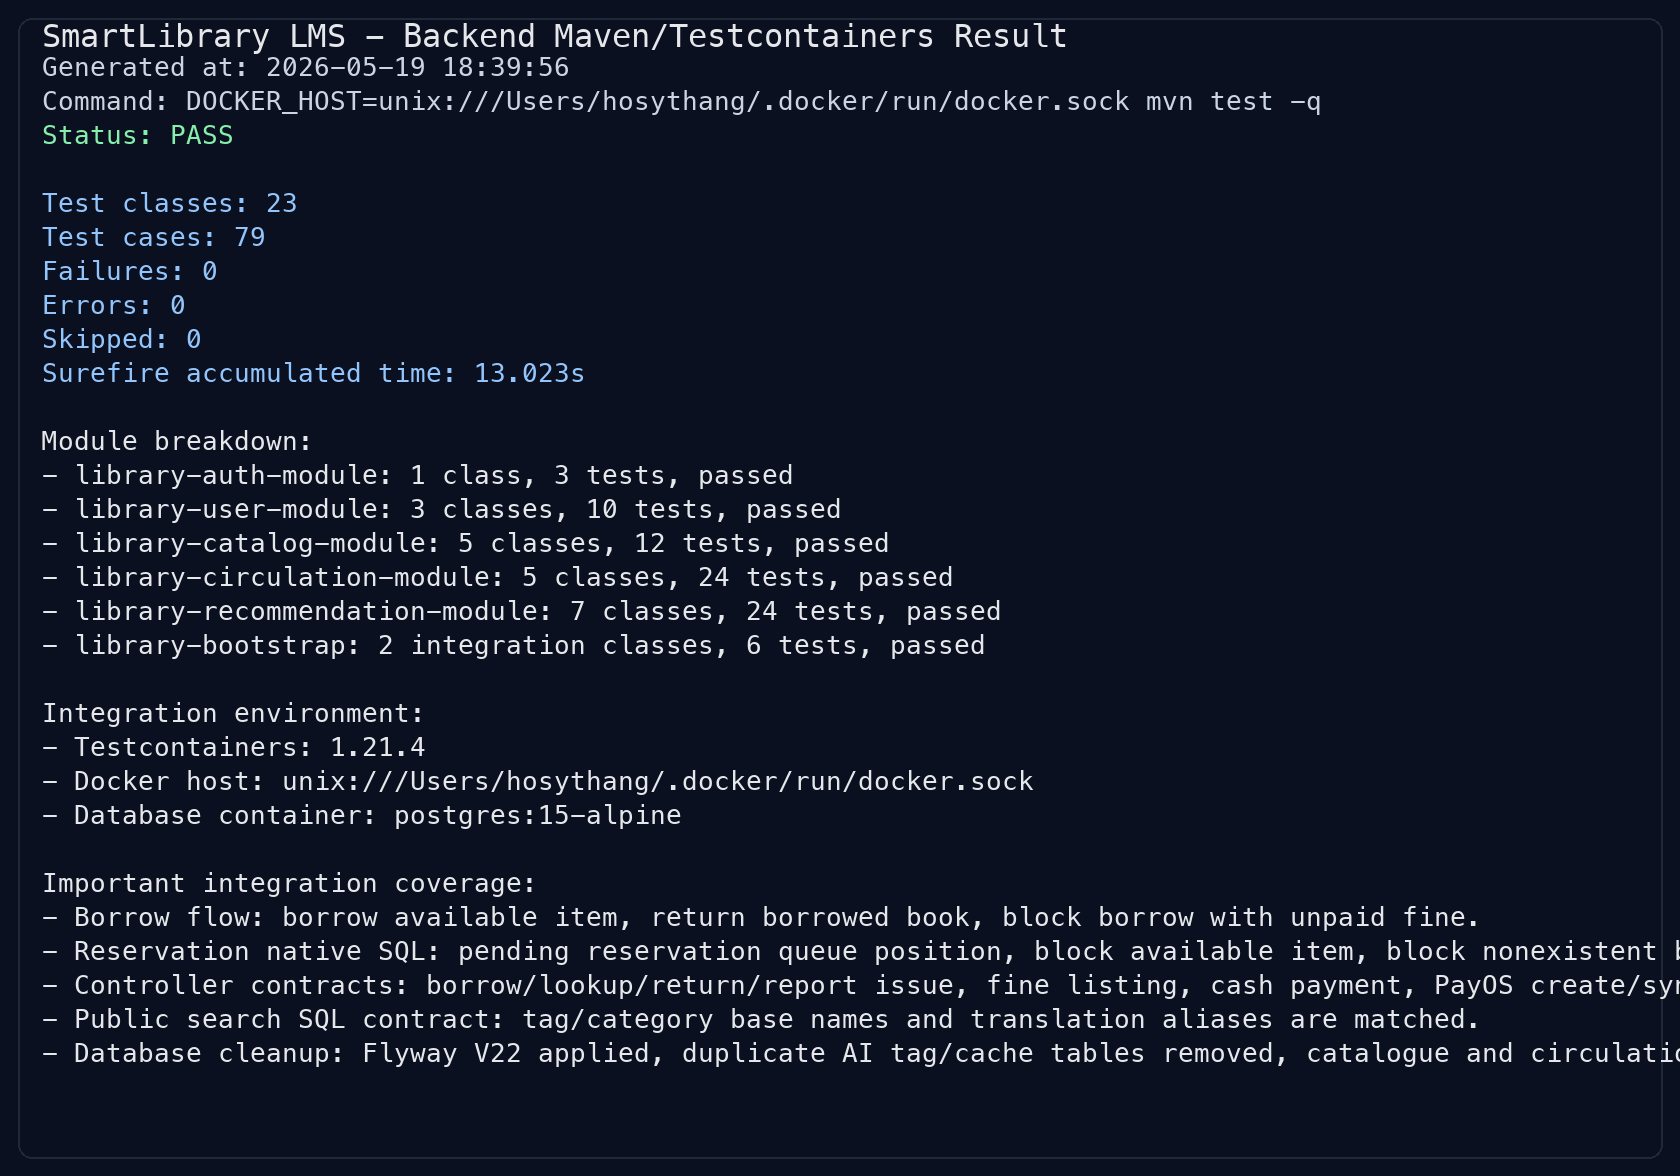
\includegraphics[width=0.9\textwidth]{figures/ch07/test-results/be-test-result.png}
    }{
        \fbox{\parbox[c][5cm][c]{0.9\textwidth}{\centering Placeholder: kết quả backend tại \texttt{figures/ch07/test-results/be-test-result.png}}}
    }
    \caption{Kết quả chạy bộ test Backend}
    \label{fig:be_test_result}
\end{figure}

\subsection{Phạm vi test Backend đã hiện thực}

Bộ test backend có 23 test class với 79 test case. Phạm vi được chọn
theo các luồng cốt lõi nhóm đã xây dựng: đăng ký/xác thực, notification, catalog
tài liệu, mượn--trả sách, đặt trước, rating/wishlist, AI gateway và callback từ
AI service. Với admin console và quy định mượn trả cấu hình từ DB, các test
circulation sử dụng mock \texttt{CirculationPolicyService}, bảo đảm unit test
phản ánh đúng cách runtime đọc policy thay vì giả định hằng số cứng.

\begin{table}[H]
\centering
\small
\begin{tabularx}{\textwidth}{|p{4.2cm}|p{2.2cm}|p{2cm}|X|}
\hline
\textbf{Module} & \textbf{Số class} & \textbf{Số test} & \textbf{Nội dung chính} \\
\hline
\texttt{library-auth-module} & 1 & 3 & Controller đăng ký, payload hợp lệ và validation email/student id. \\
\hline
\texttt{library-user-module} & 3 & 10 & Signup use case, notification page, unread count, mark read và mark all read. \\
\hline
\texttt{library-catalog-module} & 5 & 12 & Tạo publication/item, document upload URL, save document URL, public search SQL contract và publication controller. \\
\hline
\texttt{library-circulation-module} & 5 & 24 & Borrow request, return book, overdue fine, unpaid fine, borrow/reservation limit lấy từ \texttt{CirculationPolicyService}, reservation use case, transaction controller và fine/PayOS controller. \\
\hline
\texttt{library-recommendation-module} & 7 & 24 & Wishlist, rating, AI gateway fallback, semantic/recommendation contract và signed AI callback. \\
\hline
\texttt{library-bootstrap} & 2 & 6 & Integration với PostgreSQL thật: borrow/return flow và reservation native SQL. \\
\hline
\textbf{Tổng cộng} & \textbf{23} & \textbf{79} & \textbf{Toàn bộ pass}. \\
\hline
\end{tabularx}
\caption{Tổng hợp test Backend theo module}
\label{tab:be_test_modules}
\end{table}

\subsection{Kết quả thực thi Backend}

Bộ test backend cuối cùng chạy thành công toàn bộ. Kết quả chi tiết được lưu tại
thư mục \texttt{figures/test-results}, gồm file tóm tắt
\texttt{be-test-result.txt} và log Maven đầy đủ
\texttt{be-full-test-result.txt}.

\begin{table}[H]
\centering
\small
\begin{tabularx}{\textwidth}{|p{4cm}|X|}
\hline
\textbf{Chỉ số} & \textbf{Kết quả} \\
\hline
Test classes & \textbf{23}. \\
\hline
Test cases & \textbf{79 passed / 79 total}. \\
\hline
Failures & \textbf{0}. \\
\hline
Errors & \textbf{0}. \\
\hline
Skipped & \textbf{0}. \\
\hline
Thời gian Surefire & Khoảng \textbf{13.023s}. \\
\hline
Kết luận & Bộ test backend pass toàn bộ ở tầng unit/controller và integration PostgreSQL. \\
\hline
\end{tabularx}
\caption{Kết quả kiểm thử Backend}
\label{tab:be_test_result}
\end{table}

\subsection{Đánh giá và giới hạn}

Bộ test backend đã bao phủ các thành quả chính của hệ thống: quản lý
ấn phẩm, upload tài liệu, tìm kiếm public, đăng ký người dùng, notification,
mượn--trả sách, đặt trước, phí phạt/thanh toán, rating, wishlist và tích hợp AI. Đặc biệt, nhóm đã
kiểm thử integration với PostgreSQL thật bằng Testcontainers để chứng minh các
native SQL và migration hoạt động trên môi trường gần với triển khai thực tế.

Giới hạn còn lại là bộ test chưa thay thế hoàn toàn kiểm thử E2E nhiều dịch vụ
cùng lúc với frontend, backend, AI service, Kafka và PayOS sandbox đều đang
chạy. Tuy nhiên, ở phạm vi backend độc lập, bộ test đủ để chứng minh
các use case cốt lõi, controller contract và truy vấn database quan trọng hoạt
động đúng.

\section{Kiểm thử AI Service}

AI service là phần chịu trách nhiệm xử lý tài liệu PDF, tạo vector embedding,
sinh metadata học thuật, tìm kiếm ngữ nghĩa và gợi ý sách. Vì vậy nhóm không chỉ
kiểm thử API trả đúng schema, mà còn kiểm thử các ràng buộc chất lượng ở bên
trong pipeline: làm sạch PDF, chia chunk ổn định, reduce không dùng metadata
catalog để viết summary, tag tiếng Việt đúng 5 nhãn, alias tiếng Anh khớp
1--1, SQL ghi vào đúng schema \texttt{public}/\texttt{ai\_engine}, hybrid search
ưu tiên lexical trước semantic với truy vấn ngắn, recommender có fallback và
worker callback có chữ ký HMAC.

Riêng đối với phân hệ schema AI, kiểm thử giao ước dữ liệu (test contract) tập trung xác nhận pipeline thực hiện ghi nhận chính xác vào các đích lưu trữ sau:
\begin{itemize}
    \item \textbf{Dữ liệu Vector:} Ghi cấu trúc vector vào bảng \texttt{ai\_engine.publication\_vectors}.
    \item \textbf{Phân loại dữ liệu (Tags):} Định tuyến dữ liệu tag vào phân hệ chung thông qua \texttt{public.tags} và \texttt{public.publication\_tags}.
    \item \textbf{Bản địa hóa ngôn ngữ:} Lưu trữ cấu hình alias tại \texttt{public.tag\_translations}.
\end{itemize}
Đồng thời, phạm vi kiểm thử đảm bảo hệ thống hoàn toàn cô lập, không phát sinh phụ thuộc vào các bảng nằm ngoài cấu trúc schema đích bao gồm: \texttt{ai\_engine.tags}, \texttt{ai\_engine.publication\_tags} và \texttt{ai\_engine.recommendation\_cache}.

\subsection{Môi trường kiểm thử AI}

Bộ test AI được viết bằng \texttt{pytest}. Các test chính chạy offline, không gọi
Gemini thật, không cần PostgreSQL, RabbitMQ hoặc backend đang chạy. Những test
tích hợp live cho API vẫn được giữ trong thư mục \texttt{tests/integration} và
chỉ chạy khi bật biến môi trường \texttt{RUN\_LIVE\_AI\_CONTRACT\_TESTS=1}.
Cách tách này giúp nhóm có một bộ regression nhanh để chạy thường xuyên, đồng
thời vẫn có đường kiểm thử end-to-end khi cần đo latency với service thật.

\begin{table}[H]
\centering
\small
\begin{tabularx}{\textwidth}{|p{4cm}|X|}
\hline
\textbf{Thành phần} & \textbf{Cấu hình sử dụng} \\
\hline
Test runner & \texttt{pytest 8.3.5}, chạy bằng \texttt{PYTHONPATH=. ./venv/bin/python -m pytest -q}. \\
\hline
Mock LLM & Stub \texttt{GeminiClient.\_call} để trả JSON cố định, không gọi API ngoài. \\
\hline
Mock database & Fake connection/cursor để bắt SQL và tham số, không cần PostgreSQL thật. \\
\hline
Mock gateway & Monkeypatch các hàm search/recommendation để kiểm thứ tự merge, limit và fallback. \\
\hline
Mock worker & Mock Celery signal/app và HTTP request để kiểm payload, download và HMAC callback. \\
\hline
Live integration & 3 test contract/latency được skip mặc định, chỉ bật khi có AI API thật qua \texttt{AI\_API\_BASE\_URL}. \\
\hline
\end{tabularx}
\caption{Cấu hình kiểm thử AI Service}
\label{tab:ai_test_env}
\end{table}


\begin{figure}[H]
    \centering
    \IfFileExists{figures/ch07/test-results/ai-pytest-result.png}{
        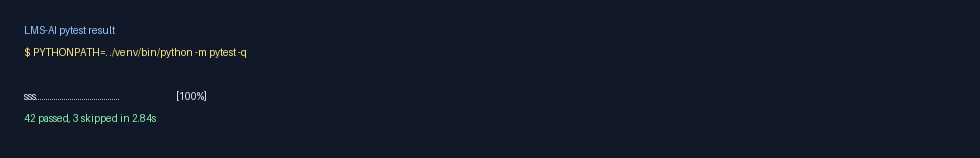
\includegraphics[width=0.9\textwidth]{figures/ch07/test-results/ai-pytest-result.png}
    }{
        \fbox{\parbox[c][5cm][c]{0.9\textwidth}{\centering Placeholder: kết quả AI pytest tại \texttt{figures/ch07/test-results/ai-pytest-result.png}}}
    }
    \caption{Kết quả chạy bộ test AI Service}
    \label{fig:ai_pytest_result}
\end{figure}

\subsection{Phạm vi test AI đã hiện thực}

Bộ test AI có 9 file test với 47 test case được collect. Trong đó 44
test offline pass và 3 test live integration được skip mặc định. Các test được
chia theo module thay vì chỉ theo endpoint, vì lỗi trong AI thường xuất hiện ở
giữa pipeline: PDF nhiễu làm chunk sai, LLM trả JSON lệch, tag bị generic, SQL
ghi sai schema hoặc hybrid search merge sai thứ tự.

\begin{table}[H]
\centering
\small % Nâng cỡ chữ lên để đọc rõ ràng, tương thích chuẩn báo cáo
\renewcommand{\arraystretch}{1.5} % Tạo không gian thở rộng rãi cho từng dòng
\begin{tabularx}{\textwidth}{|p{5.6cm}|>{\raggedright\arraybackslash}X|p{1.8cm}|}
\hline
\textbf{File test} & \textbf{Nội dung kiểm thử} & \textbf{Số test} \\
\hline
\texttt{tests/test\_ai\_metadata\_} \newline \texttt{quality.py} & Fallback tag, summary chỉ dựa trên PDF content, lọc tag generic/title/category và alias tiếng Anh. & 5 \\
\hline
\texttt{tests/test\_pdf\_processing.py} & Làm sạch header/footer/số trang, bỏ ký tự null, ghép từ bị xuống dòng, chunk id ổn định và validate \texttt{chunk\_overlap}. & 4 \\
\hline
\texttt{tests/test\_llm\_client.py} & Parse JSON từ Gemini, lỗi response rỗng, reduce metadata, lọc tag xấu, giữ alias \texttt{tags\_en} đúng cặp và reject summary kiểu catalog. & 6 \\
\hline
\texttt{tests/test\_pipeline\_core.py} & Chọn representative chunks, áp budget reduce, fallback khi LLM lỗi, optional English metadata translation và hash file/URL. & 7 \\
\hline
\texttt{tests/test\_database\_sql\_} \newline \texttt{contract.py} & SQL contract cho vector, publication tags, \texttt{public.tags}, \texttt{public.tag\_translations} và điều kiện đủ AI output. & 5 \\
\hline
\texttt{tests/test\_api\_service\_} \newline \texttt{contract.py} & pgvector literal, tokenize tiếng Việt không dấu, merge hybrid search, giới hạn \texttt{limit}, lexical-first cho query ngắn và fallback recommendation khi ALS lỗi. & 9 \\
\hline
\texttt{tests/test\_recommender\_} \newline \texttt{engine.py} & ALS bundle settings, trọng số interaction, cold user và danh sách publication id từ model recommendation. & 4 \\
\hline
\texttt{tests/test\_worker\_contract.py} & Validate payload RabbitMQ, download PDF tạm, webhook JSON compact và chữ ký HMAC \texttt{timestamp.body}. & 4 \\
\hline
\texttt{tests/integration/test\_api\_} \newline \texttt{contract\_and\_latency.py} & Health, semantic search và recommendation contract/latency với AI API thật; skip mặc định. & 3 skip \\
\hline
\textbf{Tổng cộng} & \textbf{44 pass, 3 skip} & \textbf{47} \\
\hline
\end{tabularx}
\caption{Các file test AI Service đã hiện thực}
\label{tab:ai_test_files}
\end{table}
\subsection{Kết quả thực thi AI}

Bộ test AI cuối cùng chạy thành công toàn bộ phần offline. Ba test integration
live được collect nhưng skip mặc định vì chúng yêu cầu AI API thật đang chạy và
có dữ liệu/embedding trong database.

\begin{table}[H]
\centering
\small
\begin{tabularx}{\textwidth}{|p{4cm}|X|}
\hline
\textbf{Chỉ số} & \textbf{Kết quả} \\
\hline
Test files & \textbf{9}. \\
\hline
Test cases collected & \textbf{47}. \\
\hline
Passed & \textbf{44}. \\
\hline
Skipped & \textbf{3} live integration tests. \\
\hline
Failures/Errors & \textbf{0}. \\
\hline
Thời gian chạy & Khoảng \textbf{3.94s} trên môi trường local. \\
\hline
Kết luận & Bộ test AI pass toàn bộ ở tầng unit/contract offline; test live được giữ để chạy khi có môi trường tích hợp. \\
\hline
\end{tabularx}
\caption{Kết quả kiểm thử AI Service}
\label{tab:ai_test_result}
\end{table}

\subsection{Benchmark định lượng chất lượng AI}

Để tránh đánh giá AI bằng nhận xét cảm tính, nhóm bổ sung benchmark định lượng
trên bộ dữ liệu thật \texttt{evaluation/ai\_quality\_cases.real.json}. Bộ này
gồm 6 đầu sách đã được force reprocess bằng pipeline AI hiện tại và 4 truy vấn
tìm kiếm ngữ nghĩa có ground truth thủ công. Script
\texttt{scripts/ai\_quality\_benchmark.py} đọc metadata mới nhất từ PostgreSQL,
gọi live endpoint \texttt{/api/v1/semantic-search}, sau đó tính các metric phù
hợp với từng bài toán: \texttt{Precision/Recall/F1} cho tag,
\texttt{Keyword coverage} và \texttt{Hallucination guard} cho summary,
\texttt{MRR}, \texttt{Recall@5} và \texttt{nDCG@5} cho ranking, đồng thời đo
\texttt{p50}/\texttt{p95} latency.

\begin{figure}[H]
    \centering
    \IfFileExists{figures/ch07/test-results/ai-quality-benchmark-result.png}{
        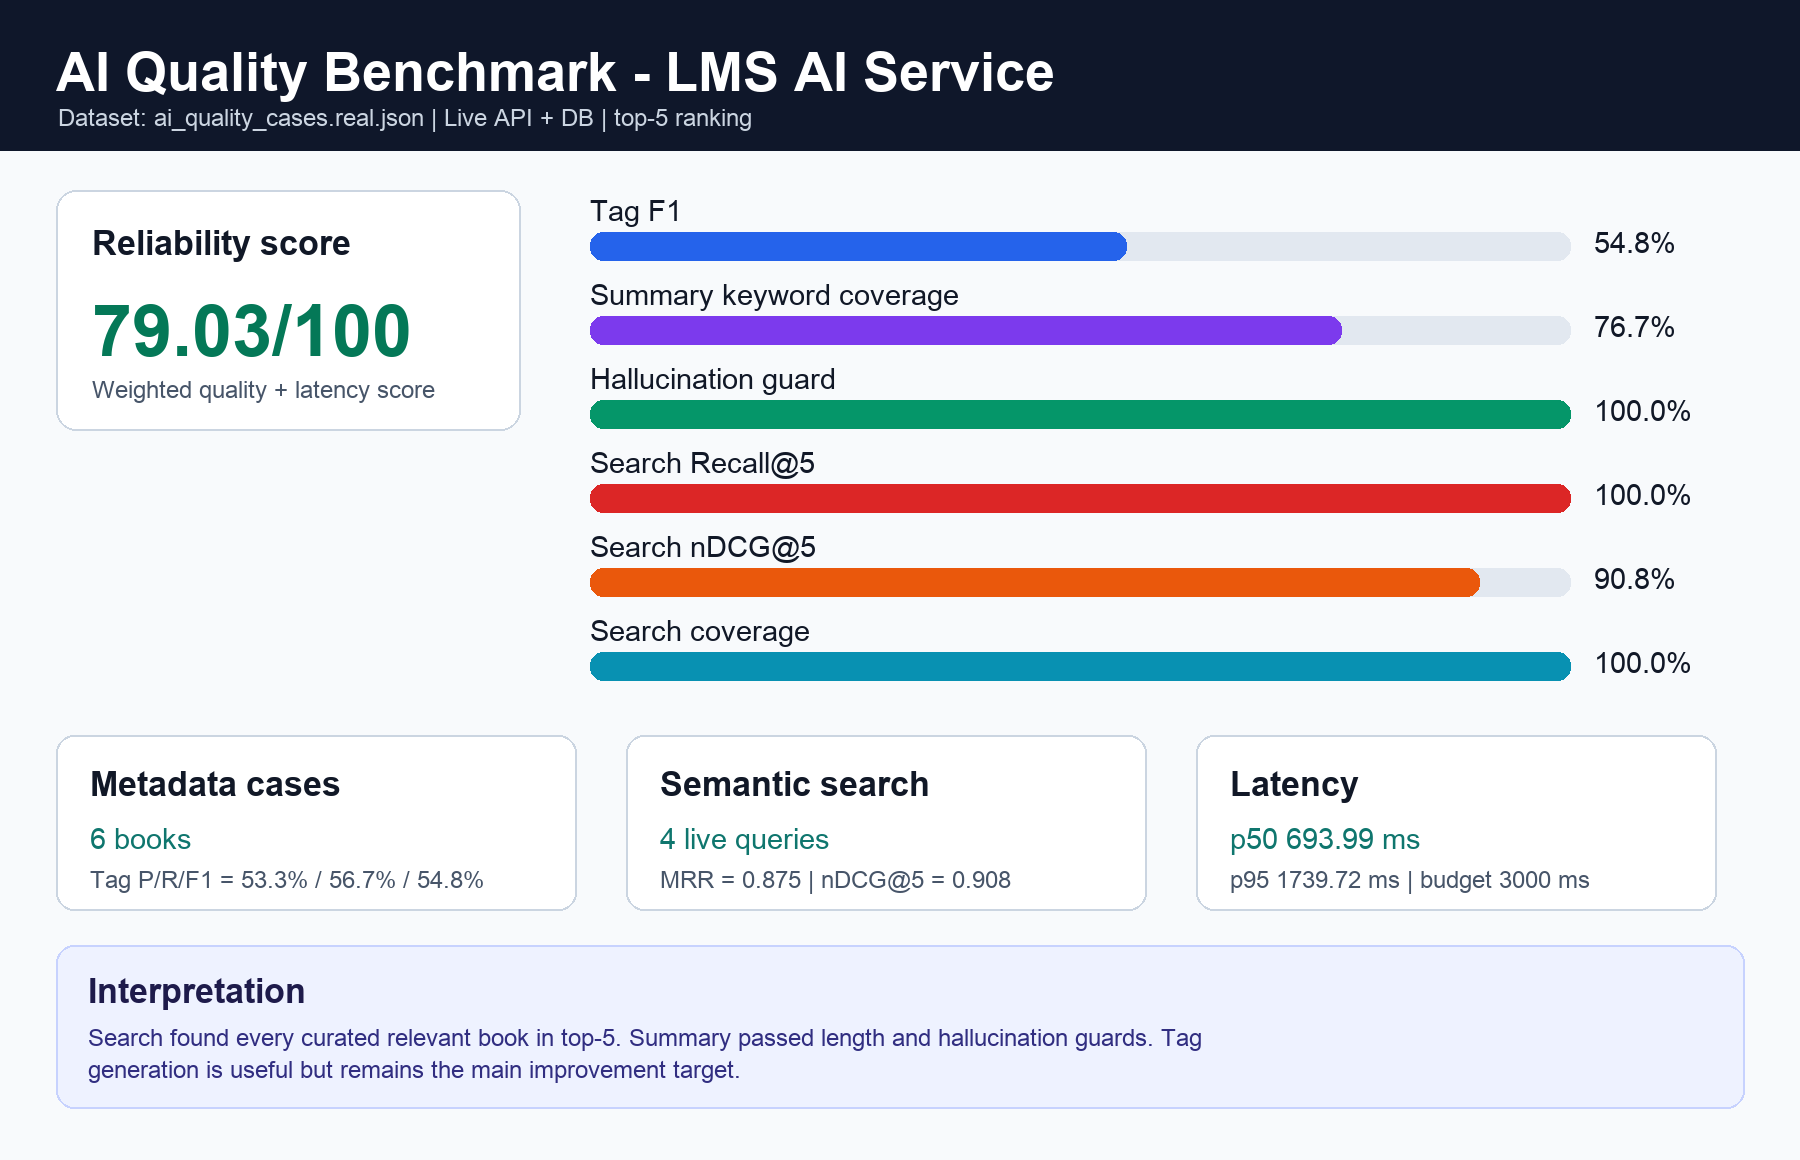
\includegraphics[width=0.95\textwidth]{figures/ch07/test-results/ai-quality-benchmark-result.png}
    }{
        \fbox{\parbox[c][5cm][c]{0.9\textwidth}{\centering Placeholder: kết quả benchmark AI tại \texttt{figures/ch07/test-results/ai-quality-benchmark-result.png}}}
    }
    \caption{Kết quả benchmark định lượng chất lượng AI trên dữ liệu thật}
    \label{fig:ai_quality_benchmark_result}
\end{figure}

\begin{table}[H]
\centering
\small
\begin{tabularx}{\textwidth}{|p{4.5cm}|X|p{2.5cm}|}
\hline
\textbf{Nhóm đánh giá} & \textbf{Metric} & \textbf{Kết quả} \\
\hline
Tổng hợp & Reliability score có trọng số từ metadata, search và latency & \textbf{79.03/100} \\
\hline
Metadata & Tag precision / recall / F1 so với tag chuẩn thủ công & \textbf{53.3\% / 56.7\% / 54.8\%} \\
\hline
Summary & Keyword coverage, length OK và hallucination guard & \textbf{76.7\%, 100.0\%, 100.0\%} \\
\hline
Semantic search & Recall@5, MRR và nDCG@5 trên 4 truy vấn live & \textbf{100.0\%, 0.875, 0.908} \\
\hline
Coverage & Tỉ lệ query trả về danh sách kết quả khác rỗng & \textbf{100.0\%} \\
\hline
Runtime & p50 / p95 latency khi gọi live AI API, budget 3000ms & \textbf{693.99ms / 1739.72ms} \\
\hline
\end{tabularx}
\caption{Kết quả benchmark AI trên bộ ground truth thật}
\label{tab:ai_quality_benchmark_result}
\end{table}

Kết quả này cho thấy phần search là điểm mạnh rõ nhất: toàn bộ truy vấn đều tìm
được sách đúng trong top 5, với \texttt{nDCG@5 = 0.908} và \texttt{MRR = 0.875},
tức là kết quả đúng thường xuất hiện rất sớm trong danh sách. Summary cũng đạt
ngưỡng an toàn tốt: độ phủ keyword đạt \textbf{76.7\%}, tất cả summary nằm trong
giới hạn độ dài và không chứa forbidden terms trong bộ kiểm thử.

Điểm cần cải thiện nằm ở sinh tag. \texttt{Tag F1 = 54.8\%} chưa đạt ngưỡng
mong muốn cho báo cáo dài hạn, nhưng đây là số liệu thật và có thể giải thích
được: một số tag đúng hướng nhưng khác cách đặt nhãn so với ground truth, và có
trường hợp sinh một tag lệch domain. Nhóm vẫn đưa chỉ số này vào báo cáo thay vì
ẩn đi, vì mục tiêu kiểm thử AI là chứng minh hệ thống được đo lường và kiểm soát
bằng số liệu lặp lại được, không phải chỉ trình bày các ví dụ đẹp.

Phần recommendation chưa được chấm trong benchmark này vì chưa có bộ user
profile ground truth được curator gán thủ công. Nếu tự gán bừa nhãn recommend để
làm đẹp điểm thì kết quả không có giá trị kiểm thử. Do đó báo cáo hiện tại chỉ
kết luận định lượng cho metadata, summary, semantic search và latency; còn
recommendation được kiểm bằng unit/contract test và cần bổ sung bộ ground truth
riêng khi có đủ dữ liệu hành vi người dùng thật.

\subsection{Đánh giá và giới hạn}

Bộ test AI đã bao phủ các tính năng chính của service: xử lý PDF,
chunking, metadata reduce, tag quality, fallback khi LLM lỗi, alias tiếng Anh,
ghi SQL đúng schema, semantic search hybrid, recommendation CBF/ALS/trending và
worker callback bảo mật. Quan trọng hơn, các test đã bắt được lỗi thật trong
pipeline PDF và align \texttt{tags\_en}, qua đó giúp chất lượng AI output ổn
định hơn trước khi demo.

Giới hạn còn lại là các test offline chưa đo chất lượng ngôn ngữ thực tế của
Gemini và chưa đo latency thật trên tập dữ liệu lớn. Vì vậy nhóm vẫn giữ 3 test
integration live để chạy khi PostgreSQL, model embedding và AI API đang hoạt
động; các test này phù hợp cho giai đoạn nghiệm thu tích hợp hoặc benchmark
riêng, còn bộ 44 test offline phù hợp để chạy thường xuyên sau mỗi lần sửa code.

\section{Kiểm thử theo yêu cầu phi chức năng}

Bên cạnh kiểm thử chức năng theo từng phân hệ, nhóm đối chiếu lại các yêu cầu
phi chức năng đã nêu ở Mục~\ref{subsec:YeuCauPhiChucNang}. Không phải mọi yêu
cầu phi chức năng đều đo được hoàn toàn bằng unit test; ví dụ tính dễ học của
giao diện vẫn cần đánh giá thủ công trong quá trình demo. Tuy nhiên, các yêu
cầu có tiêu chí kỹ thuật rõ ràng như giới hạn truy vấn, timeout, fallback,
phân quyền, chữ ký callback và cấu trúc module đều có thể được kiểm chứng bằng
test tự động hoặc test contract.

\begin{table}[H]
\centering
\scriptsize
\begin{tabularx}{\textwidth}{|p{3.1cm}|p{4.4cm}|X|p{2.1cm}|}
\hline
\textbf{Yêu cầu phi chức năng} & \textbf{Tiêu chí kiểm chứng được} & \textbf{Test/nhóm test liên quan} & \textbf{Kết quả} \\
\hline
Tính khả dụng & Các state toàn cục và helper UI phải nhất quán: ngôn ngữ, theme, thông báo, trạng thái đặt trước, lỗi nghiệp vụ và upload. & \texttt{LanguageContext}, \texttt{ThemeContext}, notification localization, \texttt{reservationUtils}, component dùng chung và service contract frontend. & 58/58 frontend pass. \\
\hline
Hiệu năng & Request có phân trang/giới hạn kết quả; truy vấn AI và recommendation không được nhận limit không kiểm soát; SQL dài có statement timeout. & Public search backend cap page size tối đa 50; AI semantic search cap \texttt{limit} theo cấu hình; recommender dùng \texttt{SET LOCAL statement\_timeout}; live latency test giữ để benchmark khi có môi trường thật. & Pass; live latency skip mặc định. \\
\hline
Độ tin cậy & Dịch vụ phụ trợ lỗi không được làm sập nghiệp vụ chính; AI/Gemini lỗi phải có fallback xác định. & AI gateway backend trả fallback khi HTTP 500; AI ETL fallback metadata khi LLM lỗi; recommendation fallback sang content-based/trending khi ALS lỗi; worker callback ghi trạng thái rõ ràng. & Pass. \\
\hline
Bảo mật & API nhạy cảm phải dựa trên JWT/role; callback/webhook phải xác thực chữ ký; upload PDF không đi qua endpoint mở tùy ý. & Auth/controller test, admin endpoint contract, PayOS webhook reject chữ ký sai, AI callback HMAC reject thiếu/sai chữ ký, frontend upload dùng presigned URL và raw axios. & Pass. \\
\hline
Khả năng bảo trì và mở rộng & Code tách theo frontend, backend module và AI service; hợp đồng giữa các service ổn định để thay đổi nội bộ không làm vỡ tích hợp. & 11 frontend suite, 23 backend test class và 9 AI test file tách theo module; service contract kiểm URL/payload; SQL contract kiểm schema \texttt{public}/\texttt{ai\_engine}. & Pass. \\
\hline
\end{tabularx}
\caption{Đối chiếu kiểm thử với yêu cầu phi chức năng}
\label{tab:nfr_test_mapping}
\end{table}

Từ bảng~\ref{tab:nfr_test_mapping}, các yêu cầu phi chức năng có khả năng
kiểm chứng bằng mã nguồn đều đã được đưa vào bộ test regression. Phần hiệu năng
ở mức unit/contract tập trung vào các ràng buộc chống quá tải như pagination,
limit và timeout; phần đo latency thật được tách thành nhóm integration live để
chỉ chạy khi có đủ backend, database, model embedding và dữ liệu mẫu. Cách tách
này giúp bộ test thường xuyên vẫn chạy nhanh, đồng thời vẫn giữ được kịch bản
nghiệm thu phi chức năng khi triển khai trong môi trường tích hợp. Các kết quả
chạy test đã được lưu thành artifact ảnh tại
\texttt{figures/ch07/test-results/} và được nhúng trực tiếp trong các mục kiểm
thử frontend, backend và AI ở phía trên, nhờ đó phần đối chiếu phi chức năng
không chỉ dừng ở mô tả mà có bằng chứng thực nghiệm đi kèm.
